\documentclass[tikz,border=0.1in]{standalone}
\usepackage{tikz}
\usetikzlibrary{positioning, arrows.meta, fit, backgrounds, calc}
\usepackage[T1]{fontenc}
\usepackage{amssymb}
\usepackage[scaled=0.95]{helvet}
\renewcommand{\familydefault}{\sfdefault}

\definecolor{miamired}{HTML}{C3142D}
\definecolor{agentblue}{HTML}{1D5FAD}
\definecolor{evalgold}{HTML}{EFDB72}
\definecolor{nonfund}{HTML}{CCC9B8}

\tikzset{
  base/.style  = {rectangle, rounded corners, draw=gray!70, ultra thick, dashed,
                  fill=gray!6, align=center, text width=3.6cm, minimum height=2.1cm,
                  font=\small, inner sep=5pt},
  trans/.style = {rectangle, rounded corners, draw=miamired, ultra thick,
                  fill=miamired!8, align=center, text width=3.0cm, minimum height=2.1cm,
                  font=\small, inner sep=5pt},
  rel/.style   = {rectangle, rounded corners, draw=agentblue, ultra thick,
                  fill=agentblue!6, align=center, text width=3.35cm, minimum height=2.1cm,
                  font=\small, inner sep=5pt},
  lab/.style   = {font=\small, align=center},
  flow/.style  = {ultra thick, -{Stealth[length=3mm]}, draw=miamired!65},
}

\begin{document}
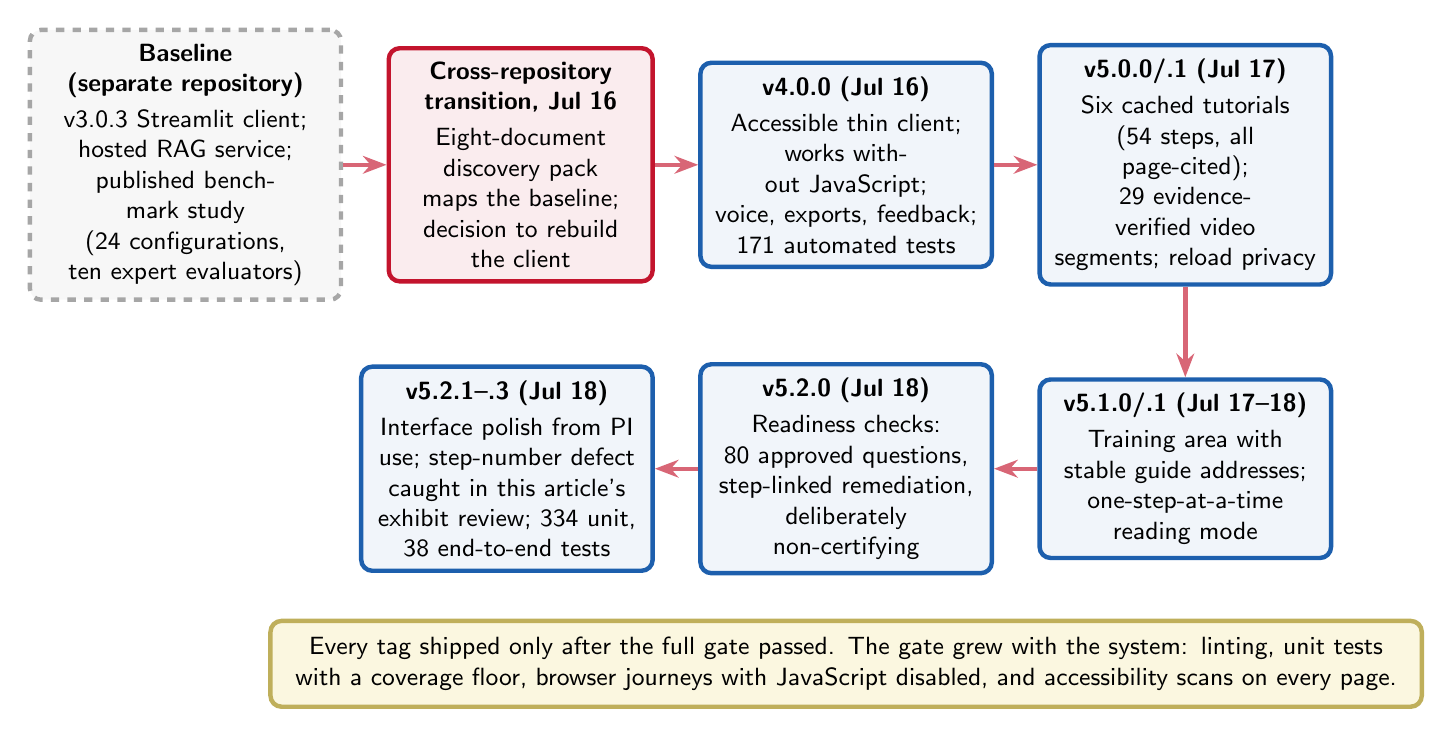
\begin{tikzpicture}[node distance=0.55cm and 0.55cm]

% Row 1: baseline, transition, first rebuild release
\node (b1) [base] {\textbf{Baseline}\\\textbf{(separate repository)}\\[2pt]
  v3.0.3 Streamlit client;\\hosted RAG service;\\published benchmark study\\(24 configurations,\\ten expert evaluators)};
\node (t1) [trans, right=of b1] {\textbf{Cross-repository transition, Jul 16}\\[2pt]
  Eight-document discovery pack maps the baseline;\\decision to rebuild\\the client};
\node (r1) [rel, right=of t1] {\textbf{v4.0.0 (Jul 16)}\\[2pt]
  Accessible thin client;\\works without JavaScript;\\voice, exports, feedback;\\171 automated tests};
\node (r2) [rel, right=of r1] {\textbf{v5.0.0/.1 (Jul 17)}\\[2pt]
  Six cached tutorials\\(54 steps, all page-cited);\\29 evidence-verified video\\segments; reload privacy};

% Row 2, right to left underneath (serpentine, matching the process figure)
\node (r3) [rel, below=1.15cm of r2] {\textbf{v5.1.0/.1 (Jul 17--18)}\\[2pt]
  Training area with\\stable guide addresses;\\one-step-at-a-time\\reading mode};
\node (r4) [rel, left=of r3] {\textbf{v5.2.0 (Jul 18)}\\[2pt]
  Readiness checks:\\80 approved questions,\\step-linked remediation,\\deliberately non-certifying};
\node (r5) [rel, left=of r4] {\textbf{v5.2.1--.3 (Jul 18)}\\[2pt]
  Interface polish from PI\\use; step-number defect\\caught in this article's\\exhibit review; 334 unit,\\38 end-to-end tests};

\draw [flow] (b1) -- (t1);
\draw [flow] (t1) -- (r1);
\draw [flow] (r1) -- (r2);
\draw [flow] (r2) -- (r3);
\draw [flow] (r3) -- (r4);
\draw [flow] (r4) -- (r5);

% Bottom band: what held constant
\node (band) [lab, below=0.55cm of r4, text width=14.2cm,
  draw=evalgold!80!black, ultra thick, fill=evalgold!22, rounded corners,
  inner sep=6pt] {%
  Every tag shipped only after the full gate passed. The gate grew with the
  system: linting, unit tests with a coverage floor, browser journeys with
  JavaScript disabled, and accessibility scans on every page.};

\end{tikzpicture}
\end{document}
